%======================================================================
\chapter{Background}
%======================================================================
\section{Hollow-Core Photonic Crystal Fiber}
\subsection{Conventional TIR Guidance}

\subsection{Photonic Crystal Bandgap}
The 1D and 2D views of the structure
\begin{figure}
	\centering
	\begin{tabular}{cc}
		\multirow{-3}[6]{*}{\subfloat[D]{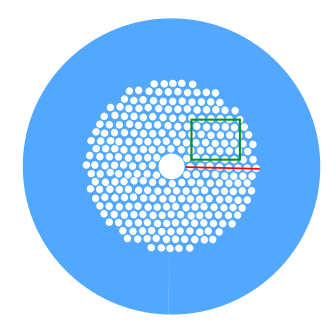
\includegraphics[width=6cm,height=6cm]{./Figures/HCPCF/HCPCF_section.png}}}&
		\subfloat[A]{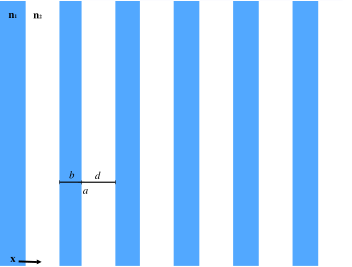
\includegraphics[width=4cm,height=3cm]{./Figures/HCPCF/HCPCF_1D.png}} \\& 
		\subfloat[H]{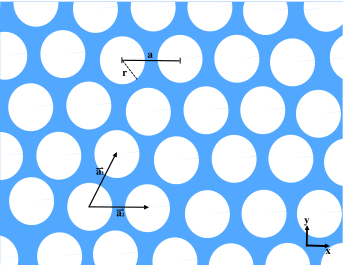
\includegraphics[width=4cm,height=3cm]{./Figures/HCPCF/HCPCF2D.png}}
	\end{tabular}
	\caption{Many figures}
	\label{fig:manyD}
\end{figure}

A periodic non-magnetic medium will have repeating dielectric constant 
\begin{equation}
	\varepsilon(\boldsymbol{r}) = \varepsilon(\boldsymbol{r}+\boldsymbol{a})  
\end{equation}
Due to its discrete and invariant translation symmetry, the dielectric constant along the medium can be expanded as a Fourier series
\begin{equation}
	\varepsilon(\boldsymbol{r}) = \sum_{\boldsymbol{G}}\varepsilon_{\boldsymbol{G}}e^{i\boldsymbol{G}\cdot\boldsymbol{r}}  
	\label{eqn:fourier_eps}
\end{equation}
Where $\boldsymbol{G}$ are the reciprocal lattice vectors such that $\boldsymbol{G}\cdot\boldsymbol{a} = 2\pi n$.Expressing the electric field also as a Fourier integral
\begin{equation}
	\boldsymbol{E}(\boldsymbol{r}) = \iiint d^3\boldsymbol{k}\boldsymbol{A}(\boldsymbol{k})e^{i\boldsymbol{k}\cdot\boldsymbol{r}}
	\label{eqn:fourier_E}
\end{equation}
 Using the Maxwell equations defined in - the wave equation can be written in terms of the electric field 
\begin{equation}
	\boldsymbol{\nabla}\times(\boldsymbol{\nabla}\times\boldsymbol{E})-\omega^2\varepsilon(\boldsymbol{r})\mu_0\boldsymbol{E} = 0
\end{equation}
Substituting \eqref{eqn:fourier_eps} and \eqref{eqn:fourier_E} into the above results in the dispersion relation:
\begin{equation}
	\boldsymbol{k}\times(\boldsymbol{k}\times\boldsymbol{A}(\boldsymbol{k})) + \omega^2\mu_0\sum_{\boldsymbol{G}}\varepsilon_{\boldsymbol{G}}\boldsymbol{A}(\boldsymbol{k}-\boldsymbol{G}) = 0
	\label{eqn:separation}
\end{equation}
in where for any vector $\boldsymbol{K}$ the solutions of \eqref{eqn:separation} for the coefficient $\boldsymbol{A}(\boldsymbol{K})$ are grouped with the coefficients $\boldsymbol{A}(\boldsymbol{K}-\boldsymbol{G})$, decoupling the coefficients of other vectors that cannot be expressed in the form $\boldsymbol{K}-\boldsymbol{G}$. Disregarding the decoupled vectors, the total electric field can be described as a superposition of normal modes with regard to a chosen vector $\boldsymbol{K}$ :
\begin{equation}
	\boldsymbol{E}_{\boldsymbol{k}}(\boldsymbol{r}) = \sum_{\boldsymbol{G}}\boldsymbol{A}(\boldsymbol{K}-\boldsymbol{G})e^{i(\boldsymbol{k}-\boldsymbol{G})\cdot \boldsymbol{r}}
	\label{eqn:normalmodes}
\end{equation}
With a little algebra, we can pull out the Bloch theorem for the electric field from \eqref{eqn:normalmodes}
\begin{equation}
	\boldsymbol{E}_{\boldsymbol{k}}(\boldsymbol{r}+\boldsymbol{a}) = e^{i\boldsymbol{k}\cdot \boldsymbol{a}}\boldsymbol{E}_{\boldsymbol{k}}(\boldsymbol{r})
\end{equation}
(Expand)  Returning to \eqref{eqn:separation}, can fix $\omega$ to find the corresponding $\boldsymbol{K}$ and normal modes os the system. However, in the case of photonic crystals there are ranges of frequencies that  have no $\boldsymbol{K}$s with real solutions, which implies that waves of these frequencies cannot propagate through the photonic crystal. These non-propagating frequencies are referred to as the photonic band gap.

\subsubsection{1D Photonic Bandgap}
Returning to the 1D periodic stack pictured in \ref{1dstack} the periodicity of dielectric constant is described by $\varepsilon(z) = \varepsilon(z+p)$ where $p = b+a$, the length of one period. The reciprocal lattice vector will be $\boldsymbol{G}_n = n\frac{2\pi}{p}\hat{z}$ and plugging into the Fourier series expansion of $\varepsilon(z)$  from \eqref{eqn:fourier_eps} 
\begin{equation}
	\varepsilon(z)  =\sum_{n=-\infty}^\infty\varepsilon_ne^{in\frac{2\pi}{p}\hat{z}}  
\end{equation}
From the reduction to propagation in the z-direction with the electric field oriented in x-direction, \eqref{eqn:separation} simplifies
\begin{equation}
K^2A(K) + \omega^2\mu_0\sum_{n=-i\infty}^\infty\varepsilon_nA(K-n\frac{2\pi}{p}) = 0
\end{equation}
Expanding the Fourier coefficients to the 1st order and reducing the equations to the dominant coefficients of the form $A(K)$ and $A(K-\frac{2\pi}{p})$ . $|K - g| = K$ and $K = \frac{\pi}{p}$ gives a system of equations that can be solved to find the dispersion relation $\omega(K)$.
\begin{equation}
	\begin{cases}
		\big(K^2-\omega^2\mu_0\varepsilon_{00}\big)A(K) = \omega^2\mu_0\varepsilon_1A(K - g)\\
		\omega^2\mu_0\varepsilon_{-1}A(K) = \big((K-g)^2-\omega^2\mu_0\varepsilon_{00}\big)A(K-g) 
	\end{cases}
\end{equation}
The equations relating these two modes has a solution at
\begin{equation}
		\big(K^2-\omega^2\mu_0\varepsilon_{00}\big)\big((K-g)^2-\omega^2\mu_0\varepsilon_{00}\big) -\big(\omega^2\mu_0\varepsilon_1\big)\big(\omega^2\mu_0\varepsilon_{-1}\big)  = 0 
\end{equation}
 noting $\varepsilon_1 = \varepsilon_{-1}^*$ and $K\approx2g$ simplifies the relationship 
 \begin{equation}
 	\big(K^2-\omega^2\mu_0\varepsilon_{00}\big)^2 -\big(\omega^2\mu_0|\varepsilon_{1}|^2\big)^2  = 0 
 \end{equation}
\begin{equation}
	\omega_{\pm}^2 = \frac{K^2}{\mu_0(\varepsilon_{00}\mp|\varepsilon_1|)}
\end{equation}
The dispersion relation has two possible solutions, which specify the top and bottom of the photonic bandgap edges, as illustrated in Fig.-  
[fig of omega v. K]
If the solving for the wavevector at a frequency between $\omega_{\pm}$, only complex solutions will exist. This means that only evanescent waves, not electromagnetic waves, propagate through the medium while the electromagnetic waves are reflected back; the medium acts as a mirror for the bandgap wavelengths.\\
This is the the phenomena that allows for HCPCF to guide certain frequencies of light - wavelengths in the bandgap are reflected by surrounding Bragg Grating confining them to the core of the fiber, while the rest are allowed to propagate through the grating. 

\subsubsection{2D Photonic Bandgap}
To understand the full picture of  light propagation in hollow-core fiber, we need to expand to the 2D case pictured in  \ref{fig:manyD}.c
primitive lattice vectors
\begin{equation}
	\boldsymbol{a}_1 = a\hat{x} \hspace{1cm} \boldsymbol{a}_2 = \frac{a}{2}\hat{x}+\frac{a\sqrt{3}}{2}\hat{y}
\end{equation}
primitive reciprocal lattice vectors $\boldsymbol{b}\cdot\boldsymbol{a} = 2\pi\delta_{ij}$
\begin{equation}
	\boldsymbol{b}_1 = \frac{2\pi}{a}\hat{x}-\frac{2\pi}{a\sqrt{3}}\hat{y} \hspace{1cm} \boldsymbol{b}_2 =\frac{4\pi}{a\sqrt{3}}\hat{y} 
\end{equation}
The reciprocal lattice vector will be $\boldsymbol{G} = n\boldsymbol{b}_1 + m\boldsymbol{b}_2$ where $n, m$ are scaling factors. 
Taking propagation in the xy-plane ($K_z=0$ and $z=0$ for simplicity), $\boldsymbol{K}=K_x\hat{x}+K_y\hat{y}$ and $\boldsymbol{r}=x\hat{x}+y\hat{y}$. The 
"In the previous two sections, we used the field patterns as our guide to understand
which aspects of two-dimensional photonic crystals lead to TM and TE band gaps.
By combining our observations, we can design a photonic crystal that has band
gaps for both polarizations. Jovanopolous"

"reciprocal lattice that is also hexagonal, but rotated relative to the original lattice by 30deg. The first Brillouin zone is defined by plotting perpendicular bisectors to the reciprocal lattice vectors. The irreducible Brillouin zone is 1/12 of the first Brillouin zone; because of the lattice symmetry, it is sufficient to only solve the Bloch modes inside this irreducible Brillouin zone. Moreover, in order to determine the photonic band gap, it is sufficient to solve the band diagram only along the edges of the green triangle. Lukin"

This region is a simple triangle with side lengths $\Gamma X = \frac{2\pi}{a\sqrt{3}}$, $\Gamma J = \frac{4\pi}{3a}$, $\Gamma J = \frac{2\pi}{3a}$ 


\subsection{Bandgap Shift}
modal magnetic field distributions satisfy:
\begin{equation}
	(\nabla^2_t + k^2n(\boldsymbol{r})^2 - \beta)\boldsymbol{H(r)} = (\nabla_t\times\boldsymbol{H(r)})\times(\nabla_t ln(n(\boldsymbol{r})^2))
\end{equation}
gives scaling law for absolute refractive index at fixed contrast
"a solution for a transverse scale represented by $\Lambda$is replicated in an identical structure with a different $\Lambda$ if the wavelength is scaled proportionately, to keep $k\Lambda$ constant"
Scaling law for the wave equation for the transverse coordinates
$X=x\Lambda^{-1}$ $Y=y\Lambda^{-1}$
where $\Lambda$ is a solution to the transverse scale. 
\begin{equation}
	n(X, Y) = \begin{cases}
		1, &n_1 \text{   (high RI)}\\
		0, & n_2 \text{   (low RI)}
	\end{cases}
\end{equation}
normalized scaled wave equation:
\begin{equation}
	\nabla_\perp^2\Psi + (v^2n(X, Y) - w^2)\Psi = 0
\end{equation}
With $\nabla_\perp = \partial^2/\partial X^2 + \partial^2/\partial Y^2 $
solving for the frequency parameter $v^2$ and eigenvalue $w^2$:
\begin{equation}
	\begin{aligned}
		v^2  &= \Lambda^2k^2(n_1^2 - n_2^2)\\
		w^2 &= \Lambda^2(\beta^2 - k^2n_2^2)
	\end{aligned}
\end{equation}
from the equation above we see that the $w^2$ is determined by the frequency parameter$v^2$ and the index distribution function $n(X, Y)$. This implies that $w^2$ and $v^2$ are invariant with changes to the parameters $k, \Lambda, n_1, n_2$. 
$k = \omega/c$ $\beta = kcos\theta$ longitudinal component of the wavevector. Because the light propagates along the fiber, much of its wavevector is taken up by the longitudinal component. 

In the HCPCF case where the glass refractive index is held constant and the air in the fiber is replaced by a new material the equations can be rewritten with $n1 = n_{glass}$ and $n_2 = n_{air}=1$:
\begin{equation}
	\begin{aligned}
		v^2 - w^2 &= \Lambda^2(k^2n_{glass} - \beta^2)\\
		v &= k\Lambda n_{glass}\sqrt{n_{air} - \frac{n_{air}}{n_{new}}}
	\end{aligned}
\end{equation}
The initial index contrast $N_0 = \frac{n_{air}}{n_{glass}}$ moves to$ N = \frac{n_{new}}{n_{glass}}$ with the change in RI $n_{air} <  n_{new} < n_{glass}$
This leads to the new center bandgap to be governed by the equation: 
\begin{equation}
	\lambda = \lambda_0\sqrt{\frac{1-N^{-2}}{1-N_0^{-2}}}
\end{equation}

"We emphasise that the scalar wave equation (and therefore the scaling laws derived from it) is accurate for the smallest index contrasts only. However, for step-index structures the vector term in Eq. (2) only exists at boundaries, so the scalar wave equation accurately represents wave propagation elsewhere. Since bandgaps arise from interference and resonance effects among such generic waves, the scaling laws of Eq. (5) should be at least approximately valid" ~1.45 RI contrast

\subsection{Mode Distribution}
a) For a two-level atom, the coupling constant -- g -- [Eq. 2.6] scales inversely to this 'effective mode area'  [Eq. before 2.1]  (in the interaction energy term between atom and the field).  mode is like a Gaussian [given by the mode function f(x,y) ] the photon interacts more strongly if the atom is placed in the center of the mode.)\\
effective mode area:
\begin{equation}
	A = \frac{\int dxdy|f_k(x, y)|^2}{|f_k(x_a, y_a)|^2}
\end{equation}
where $f_k(x,y)$ is the transverse mode function and $(x_a,y_a )$ is the position of the atom, is approximately constant in the range of the relevant longitudinal wave numbers\\
coupling constant:
\begin{equation}
	g_\omega = \sqrt{\frac{\omega}{4\pi\epsilon\hbar c A}}d_{eg}
\end{equation}
(2.5) dipole interaction Hamiltonian 

b) Apparently, this coupling constant term tells us parameters such as:\\
i) how likely it is for an excitation in the emitter is released into the waveguide mode $\gamma_{1D}$, versus free-space $\gamma_0$. \cite{mazoni}
\begin{equation}
	\gamma_{1D} = 2\pi g^2_{\omega_A}  = \frac{\sigma_A}{2A}\gamma_0
\end{equation}
"where the second expression directly exhibits the scaling with the transverse extension of the waveguide. It is related to the atomic radiative cross section $\sigma_A = \frac{3\lambda^2}{2\pi}$. A natural lower bound on the transverse mode size is at about $A \sim (\frac{\lambda}{2})^2$. (lowest-order mode in hollow metallic wave- guide), implying a maximum achievable coupling ratio $\gamma_{1D}/\gamma_0 \sim 1$. In the range $\sigma_A \sim A$, one has a strong waveguide-atom coupling, which is manifested by the fact that the atom dissipates its energy equally into the waveguide and the free-space ‘‘lossy’’ modes."\cite{domokos}

ii) optical depth (OD) for a single atom is (about) the ratio of $ (\gamma_{1D})/ (\gamma_{0})$ or the ratio of the cross-section area of the atom to that of the effective mode-area. 
\begin{equation}
 	OD = \frac{\sigma_A}{\sigma_M} = \frac{\gamma_{1D}}{\gamma_0}
\end{equation}

c) OPTICAL DEPTH CALCULATIONS: Optical depth (OD) tells about how opaque the system is. Transmitted intensity goes by $T = exp(-OD)$. Normally, N emitters might scale linearly to give an optical depth ~$N*OD$. But now (due to its position) each emitter might have its own mode area.\\

Examples of taking this into account (with maybe slightly different conventions) for atoms are mentioned in these two references\cite{bajcsy, hilton}: 
\begin{equation}
	OD_{fiber} = \int^L_0 \int^{r}_0 n(\rho, z) OD 2\pi \rho d\rho dL
\end{equation}
$r$ and $L$ represent the radius and length of the ensemble, which in the case of solution-filled HCPCF is the radius and length of the fiber. This assumes that the particulates outside of the core do not have a significant contribution.  If the distribution of molecules is take to be uniform along the fiber length and radius of the core, then the number density will be: 
\begin{equation}
	n(\rho, z) = \begin{cases}
		0, &|z| > L/2\\
		(1/L) (1/\rho), &|z| < L/2
	\end{cases}
\end{equation}

\begin{thebibliography}{hcpcf}
	\bibitem{domokos} P. Domokos, P. Horak, and H. Ritsch, “Quantum description of light-pulse scattering on a single atom in waveguides,” Phys. Rev. A, vol. 65, no. 3, p. 033832, Mar. 2002, doi: 10.1103/PhysRevA.65.033832.
	
	\bibitem{solano} P. Solano et al., “Optical Nanofibers: a new platform for quantum optics,” vol. 66, 2017, pp. 439–505. doi: 10.1016/bs.aamop.2017.02.003.\\
	
	\bibitem{mazoni} M. T. Manzoni, “New Systems for Quantum Nonlinear Optics,”. 2017, Thesis, p. 39-40.
	
	\bibitem{bajcsy} M. Bajcsy et al., “Laser-cooled atoms inside a hollow-core photonic-crystal fiber,” Phys. Rev. A, vol. 83, no. 6, p. 063830, Jun. 2011, doi: 10.1103/PhysRevA.83.063830. \\
	\bibitem{hilton} A. P. Hilton, C. Perrella, F. Benabid, B. M. Sparkes, A. N. Luiten, and P. S. Light, “High-efficiency cold-atom transport into a waveguide trap,” Phys. Rev. Applied, vol. 10, no. 4, p. 044034, Oct. 2018, doi: 10.1103/PhysRevApplied.10.044034. A
\end{thebibliography}